\documentclass[14pt,a4paper]{scrartcl}
\usepackage[utf8]{inputenc}
\usepackage[english,russian,ukrainian]{babel}
\usepackage{indentfirst}
\usepackage{misccorr}
\usepackage{graphicx}
\usepackage{xcolor}
\usepackage{cmap}
\usepackage{amsmath,amsfonts,amssymb,amsthm,mathtools}
\usepackage{icomma}
\usepackage{multirow}
\usepackage{geometry} \geometry{verbose,a4paper,tmargin=1cm,bmargin=2.5 cm,lmargin=2cm,rmargin=1cm}
\usepackage{euscript}
\usepackage{mathrsfs}
\usepackage{mathtext}
\usepackage{hyperref}
\usepackage{booktabs}
\usepackage{color}
\usepackage{rotating}
\usepackage{pdflscape}
\usepackage{floatrow,subcaption,graphicx,calc}
\usepackage{tikz}
\usetikzlibrary{shapes.geometric, arrows}
\usepackage[siunitx]{circuitikz}
\linespread{1.3}
\setlength{\parindent}{5ex}


\begin{document}

\pagecolor{white}
\begin{titlepage}
  \begin{center}
    \large
    Національний технічний університет України \\ "Київський політехнічний інститут імені Ігоря Сікорського"
     
       
    Факультет Електроніки
     
    Кафедра мікроелектроніки
    \vfill
      
    \textsc{\Large Розрахуноково-графічна робота}\\
     
    {з дисципліни: «Схемотехніка-1. Аналогова схемотехніка»\\[1cm]
      
    {\bf «Синтез активних RC-фільтрів»}\\

{\large варіант \No5}
    
    }
  \bigskip
\end{center}
\vfill
 
\newlength{\ML}
\settowidth{\ML}{«\underline{\hspace{0.4cm}}» \underline{\hspace{2cm}}}
\hfill
\begin{minipage}{1\textwidth}
Виконав:\\
Студент 3-го курсу \hspace{4cm} $\underset{\text{(підпис)}}{\underline{\hspace{0.2\textwidth}}}$  \hspace{1cm}Мнацаканов А.С.\\
\vspace{1cm}

Перевірила: \hspace{6.1cm} $\underset{\text{(підпис)}}{\underline{\hspace{0.2\textwidth}}}$  \hspace{1 cm}Голубєва І.П.\\

\end{minipage}

\vfill

\begin{center}
2021
\end{center}
\end{titlepage}



\section{Завдання}
\begin{trivlist}
\item1. Визначити параметри специфікації для синтезу активного RC-фільтра. Обрати тип
фільтру у відповідності до варіанту табл. 1, тип апроксимації АЧХ обрати у відповідності
до табл. 2, числові параметри відповідно до табл. 3.
\item2. Визначити необхідний порядок фільтру та записати аналітичний вираз для функції
передачі фільтру у загальному вигляді.
\item3. Записати аналітичний вираз функції передачі фільтру у вигляді послідовно з’єднаних
ланок другого порядку в загальному вигляді.
\item4. Розрахувати коефіцієнти функції передачі фільтру.
\item5. Обрати структури фільтрів для реалізації ланок другого порядку.
\item6. Розробити принципову електричну схему активного RC-фільтру для кожної ланки другого
порядку (провести аналітичний розрахунок секцій другого порядку, провести розрахунки
номіналів схеми, обрати елементну базу).
\item7. Оформити повну схему електричну принципову розробленого фільтра у відповідності до
вимог ЕСКД.
\item8. Провести аналіз розробленої схеми. Побудувати АЧХ та ФЧХ розробленого фільтра.
Впевнитися у відповідності параметрів розробленого фільтра вимогам специфікації.
\end{trivlist}
\newpage

Тип: N1=1-ФВЧ (Фільтр верхніх частот)\\

Апроксимація: Батерворта\\

Коефіцієнт передачі у смузі пропускання: Gain=3 dB\\

fp: 4 kHz\\

fs: 1.33 kHz\\

Рівень пульсації у смузі пропускання: Rp=6 dB\\

Мінімальне подавлення у смузі затримки: Rs=22 dB\\
\newpage

Скористаймося програмою MATLAB для знаходження порядку фільтра та коефіцієнтів функції передачі:

\begin{verbatim}
n=1;
Rp=6; 
Rs=22; 
fp=4e+3;
fs=1.33e+3;
wp=2*pi*fp;
ws=2*pi*fs;
[n,wn]=buttord(wp,ws,Rp,Rs,'s');
disp(n);
[b,a]=butter(n,wp,'high','s');
disp(b(1));
disp(b(2));
disp(b(3));
disp(a(1));
disp(a(2));
disp(a(3));
\end{verbatim}

\begin{figure}[!h]\TopFloatBoxes\CenterFloatBoxes
\ffigbox{\caption{Результат роботи програми}}
{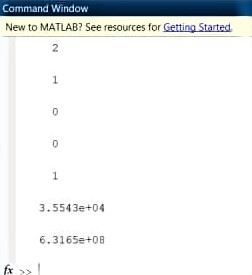
\includegraphics[width=0.3\textwidth]{prog_result}}
\end{figure}
\newpage
З допомогою MATLAB ми визначили наступні параметри:
\begin{center}
Порядок фільтру $n=2$\\[0.5cm]
$b(1)=1$, $b(2)=0$, $b(3)=0$\\[0.5cm]
$a(1)=1$, $a(2)=3,5543\cdot{10^4}$, $a(3)=6,3165\cdot{10^8}$
\end{center}

Функція передачі в загальному вигляді виглядає наступним чином:
\begin{equation}
K_U(p)=\dfrac{B(p)}{A(p)}=\dfrac{b(1)\cdot p^n+b(2)\cdot p^{n-1}+...+b(n+1)}{a(1)\cdot p^n+a(2)\cdot p^{n-1}+...+a(n+1)}.
\end{equation}

Перепишемо її, врахувавши максимальний порядок $n=2$:
\begin{equation}
K_U(p)=\dfrac{b(1)p^2+b(2)p+b(3)}{a(1)p^2+a(2)p+a(3)},
\end{equation}

Запишемо вираз функції передачі з урахуванням знайдених коефіцієнтів та коефіцієнта підсилення в смузі пропускання ($Gain=3$ дБ $=1,413$ рази):

\begin{equation}
K_U(p)=1,413\times\dfrac{p^2}{p^2+3,5543\cdot{10^4}\cdot p+6,3165\cdot{10^8}}
\end{equation}

Підберемо таку структуру фільтра аби вона задовольняла нашому виразу для $K_U(p)$. Для цього зручно буде обрати каскадне з'єднання {\bf схеми Рауха} інвертуючого ФВЧ-2 порядку та інвертуючого масштабуючого підсилювача, аби забезпечити необхідне підсилення.

\begin{figure}[!h]\TopFloatBoxes\CenterFloatBoxes
\ffigbox{\caption{Схема рауха інвертуючого ФВЧ-2 та масштабуючого підсилювача}}%
           {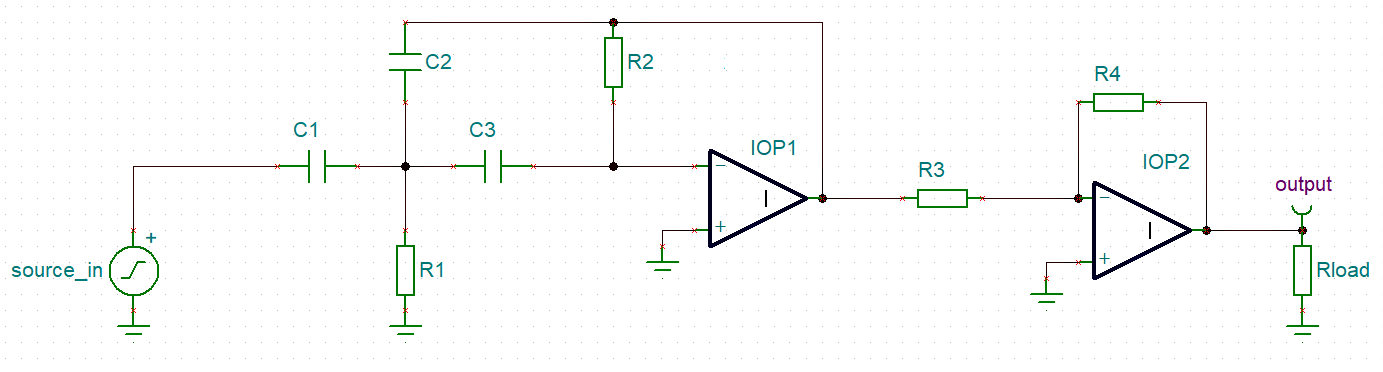
\includegraphics[width=\textwidth]{rauh}}
\end{figure}
\newpage
Запишемо вирази $K_U(p)$ послідовно з'єднаних ланок:
\begin{equation}\label{for}
K_{U_{\sum}}(p)=K_{U1}(p)K_{U2}(p)=-\dfrac{R_4}{R_3}\times-\dfrac{C_1C_3\cdot p^2}{C_2C_3\cdot p^2+G_2(C_1+C_2+C_3)\cdot p+G_2G_1}
\end{equation} 

Модифікуємо формулу \eqref{for} наступним чином:
\begin{center}
$K_U(p)=\dfrac{R_4}{R_3}\times\dfrac{C_1C_3\cdot p^2}{C_2C_3\left[p^2+\dfrac{G_2(C_1+C_2+C_3)}{C_2C_3}\cdot p+\dfrac{G_2G_1}{C_2C_3}\right]}$
\end{center}

Спростивши, отримали два остаточні вирази для $K_U(p)$:

\begin{equation}
\boxed{
\begin{aligned}
K_U(p)=\left(\dfrac{R_4}{R_3}\cdot\dfrac{C_1}{C_2}\right)\times\dfrac{p^2}{p^2+\dfrac{G_2(C_1+C_2+C_3)}{C_2C_3}\cdot p+\dfrac{G_2G_1}{C_2C_3}}\\[0.5cm]
K_U(p)=1,413\times\dfrac{p^2}{p^2+3,5543\cdot{10^4}\cdot p+6,3165\cdot{10^8}}
\end{aligned}}
\end{equation}


Прирівняємо між собою коефіцієнти, записавши наступну систему рівнянь:

\begin{equation*}
\begin{cases}
\dfrac{R_4}{R_3}\cdot\dfrac{C_1}{C_2}=1,413\\[0.5cm]
\dfrac{G_2(C_1+C_2+C_3)}{C_2C_3}=3,5543\cdot{10^4}\\[0.5cm]
\dfrac{G_2G_1}{C_2C_3}=6,3165\cdot{10^8}
\end{cases}
\end{equation*}

\begin{itemize}
\item нехай $C_1=C_2=C_3=C=1$ нФ.
\item з другого рівняння знаходимо $G_2$ як:
\begin{center}
$G_2=\dfrac{3,5543\cdot{10^4}\times C^2}{3C}=\dfrac{3,5543\cdot{10^4}\times \left(10^{-9}\right)^2}{3\cdot{10^{-9}}}=1,185\cdot{10^{-5}}$ См.
\end{center}
\item з третього рівняння знаходимо $G_1$ як:
\begin{center}
$G_1=\dfrac{6,3165\cdot{10^8}\times{C^2}}{G_2}=\dfrac{6,3165\cdot{10^8}\times{\left(10^{-9}\right)^2}}{1,185\cdot{10^{-5}}}=5,33\cdot{10^{-5}}$ См.
\end{center}
\item з першого рівняння при $C_1=C_2=C_3=C=1$ нФ маємо $\dfrac{R_4}{R_3}=1,413$, тому нехай $R_4=1413$ Ом, $R_3=1000$ Ом.
\end{itemize}
\newpage
Отже наші номінали компонентів наступні:
\begin{itemize}
\item $R_1=18,76$ кОм.
\item $R_2=84,39$ кОм.
\item $R_3=1$ кОм.
\item $R_4=1,413$ кОм.
\item $C_1=C_2=C_3=1$ нФ.
\end{itemize}
\medskip\hrule\medskip
\begin{figure}[!h]
\ffigbox{\caption{Схема рауха інвертуючого ФВЧ-2 та масштабуючого підсилювача з розрахованими номіналами}}%
           {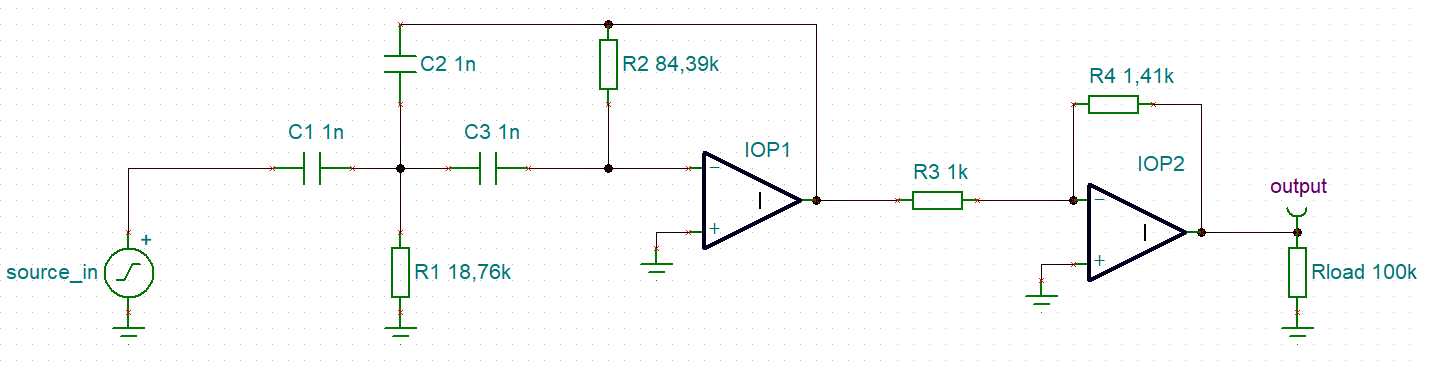
\includegraphics[width=\textwidth]{rauh1}}
\end{figure}

Побудуймо АЧХ та ФЧХ нашого фільтру:
\begin{figure}[!h]\TopFloatBoxes\CenterFloatBoxes
\ffigbox{\caption{АЧХ (зверху) та ФЧХ (знизу) фільтра}}%
           {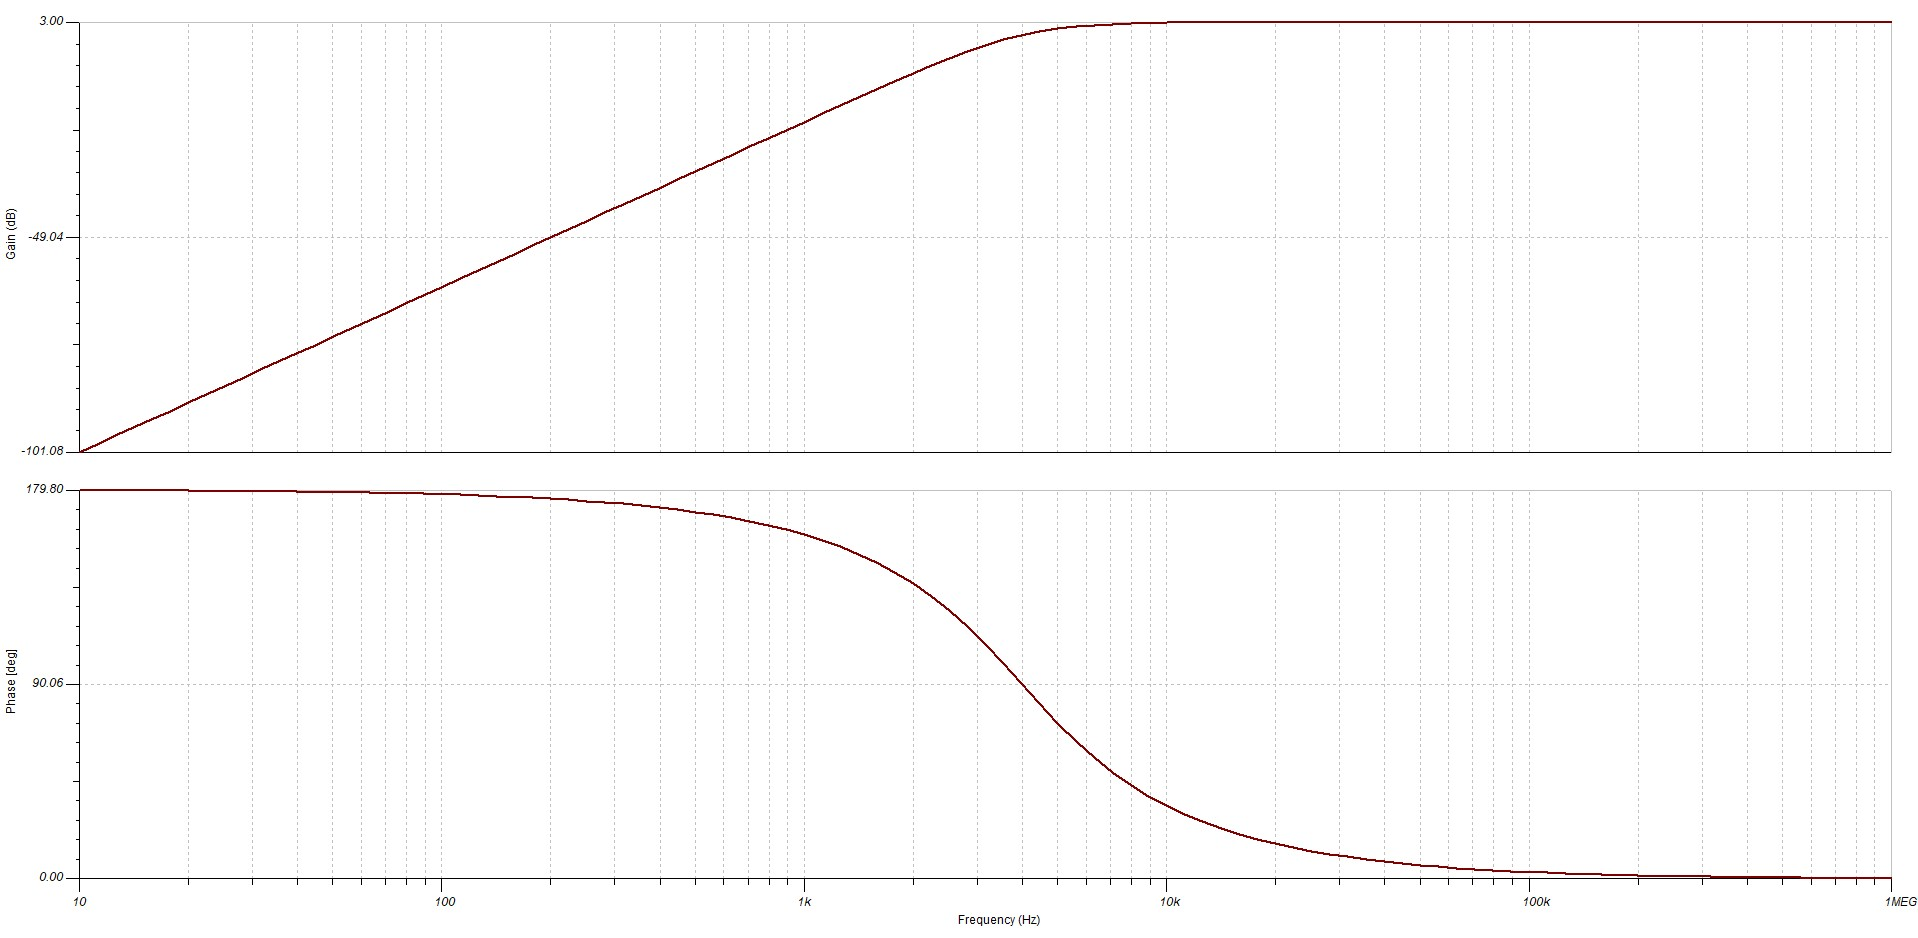
\includegraphics[width=\textwidth]{req}}
\end{figure}
\newpage
Розглянемо більш детально амплітудну характеристику:
\begin{figure}[!h]\TopFloatBoxes\CenterFloatBoxes
\ffigbox{\caption{АЧХ фільтра}}%
           {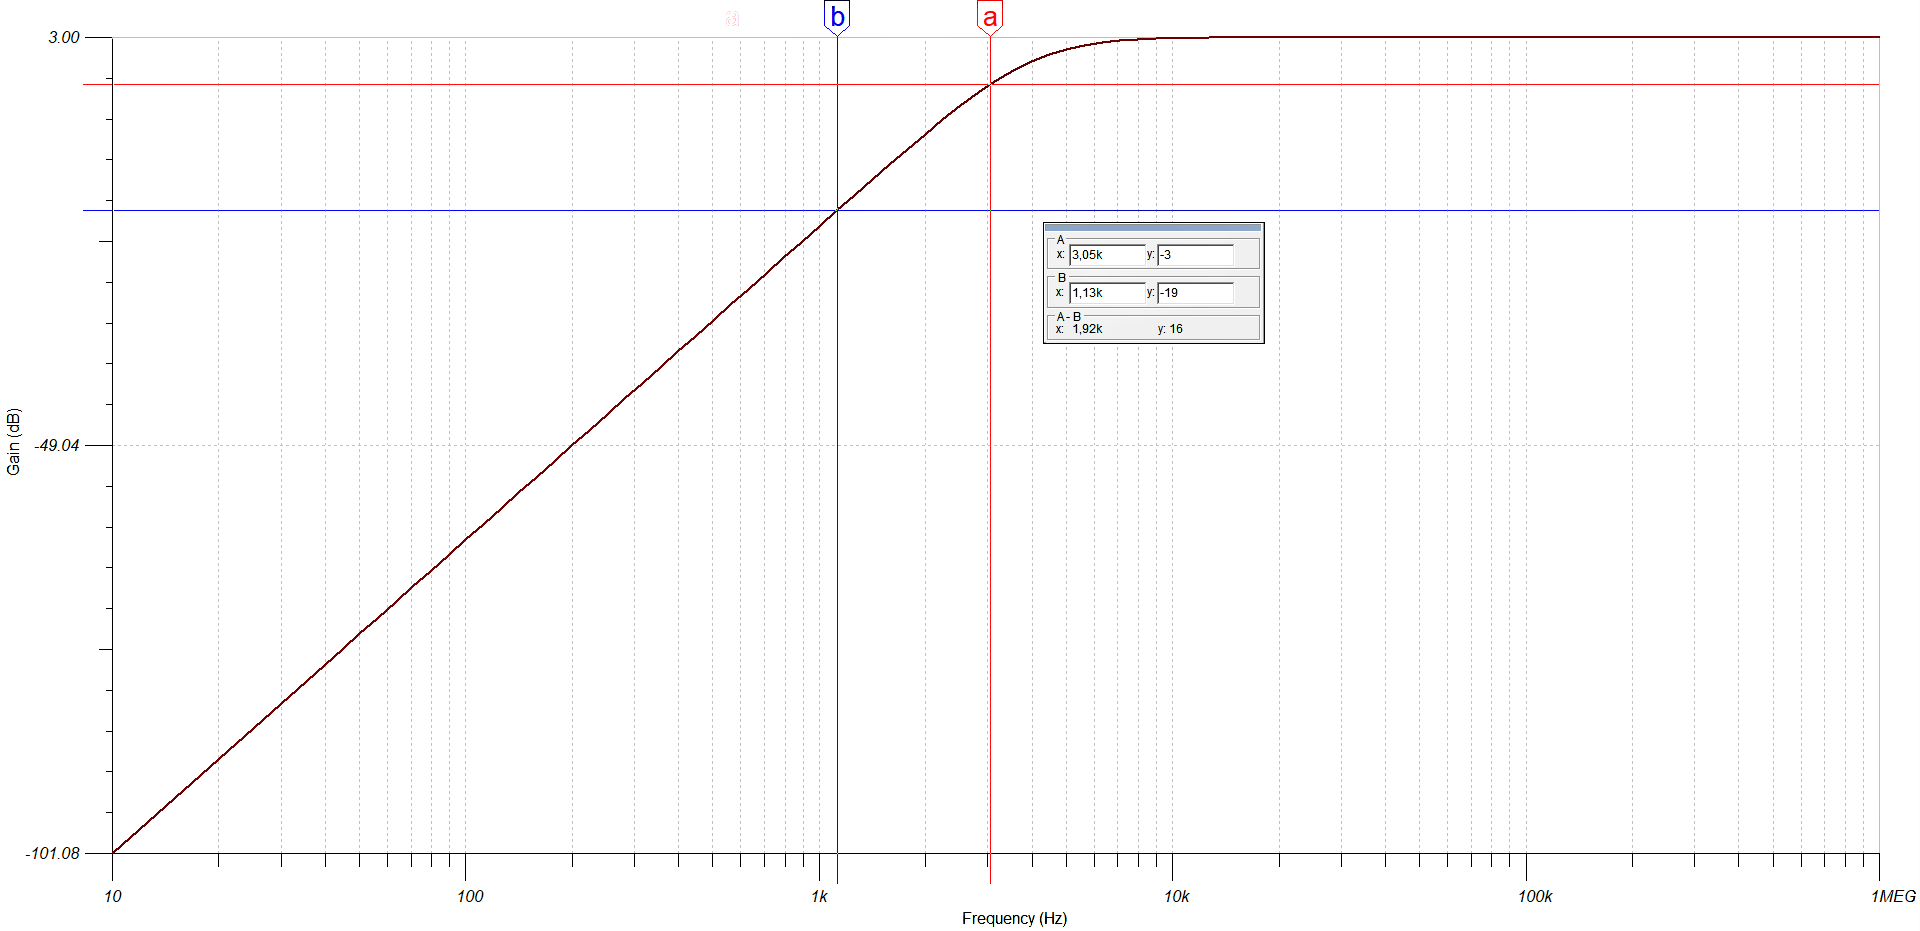
\includegraphics[width=\textwidth]{amplitude}}
\end{figure}

В специфікації було сказано, що коефіцієнт передачі в смузі пропускання має становити 3 дБ, що ми і можемо спостерігати на графіку- підсилення в 3 дБ наявне. Розглянемо вертикальний червоний маркер $a$, що відтинає на осі $Gain (dB)$ рівень -3 дБ. Як ми пам'ятаємо з умов специфікації, рівень пульсації в смузі пропускання становить 6 дБ, тобто значеня в -3 дБ (3-6) має спостерігатись на частоті $f_p=4$ кГц. На графіку ж значення $f_p=3,05$, тобто відносна похибка $\delta$ склала $31,15\%$. Розглянувши вертикальний червоний маркер $b$, що відтинає рівень -19 дБ, ми бачимо що фактична частота $f_s$ складає 1,13 кГц, що доволі непогано відповідає умовам специфікації ($f_s=1,33$ кГц), відносна похибка тут складає всього $17,7\%$.\\

Розглянувши ФЧХ нашого фільтру, ми бачимо, що вона є зеркально протилежною до теоретичних викладок, але це можна пояснити наявністю в ланці додаткового інвертуючого масштабуючого підсилювача.  






%\TopFloatBoxes\CenterFloatBoxes
%\begin{landscape} 
%\end{landscape}
%\multirow{объединить Х строк}{ширина}{содержимое}
%\begin{tabular}{|p{6cm}|p{5cm}|p{5cm}|}
%\includegraphics[width=0.5\textwidth]{lablub}
%\medskip\hrule\medskip
%\multicolumn{2}{c|}{Диаметр}

\end{document}